\section{What the adapted models have given}

The repaired models are instruments for the lunar climate, and their first products are sensitivities: how
far each Earth assumption, once removed, moves the climate, and where the uncertainty that remains now sits.
Every climate number below is a conditional model result, holding given the scenario and the Earth-fitted
parts each model keeps.

\textbf{What each repair moved.} Figure~\ref{fig:repairs} sets each repair's effect on the global-mean
surface temperature beside the sensitivity tests, each pair of runs averaged over set years and several
still drifting. On the first design run, with 25\% seas under the undimmed shield, counting cloud water by
pressure warmed the Moon by 2.3~K over the years averaged and about 2.5~K as the run settled, and counting
convective rain per Earth day warmed it by a further 1.8~K, about 1.6~K settled.\claim{G01} The Sun clock,
the Moon's own tilt and the recalibrated split of sunlight warmed it by only 0.6~K, yet cut its rain from
2.91 to 2.24~mm per day and raised the share of land receiving under 0.5~mm per day from 9 to
42\%.\claim{G02} The curved air cooled it by 0.65~K, its clouds giving back in the first year 3.5 of the
5.4~W\,m$^{-2}$ that the geometry took from the clear sky, and the carbon dioxide and oxygen bands cooled it
by a further 2.2~K, mostly through PlaSim's high cloud, since a cloud-free column moves its ground only
0.57~K: the high deck fell from 16 to 12\% of the sky, the top layer's cirrus from 2.0 to 0.05\% as that
layer warmed by 7~K.\claim{G03} Held at the design temperature by dimming the sunlight 3.0\% in place of the
earlier 5\%, the corrected Moon settles at 295.0~K, with 2.31~mm of rain a day.\claim{G04}

\begin{figure}[tbp]
\centering
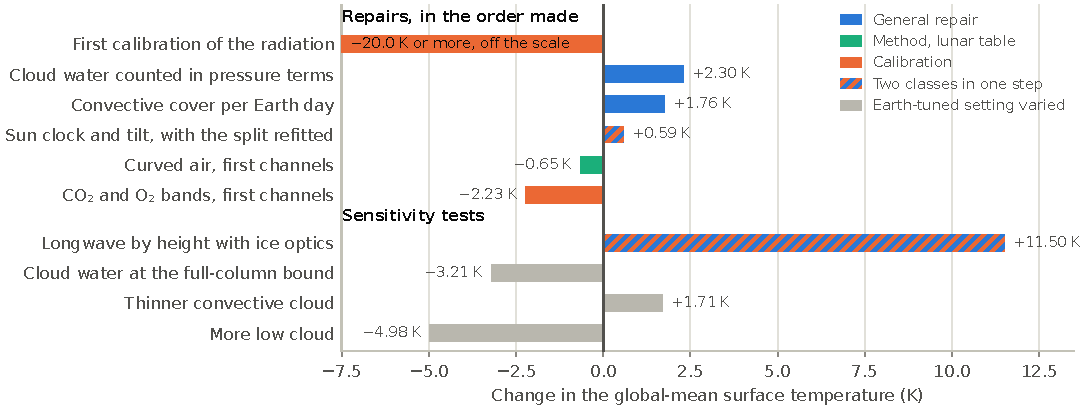
\includegraphics[width=\textwidth]{figures/fig_repairs.pdf}
\caption{Change in the global-mean surface temperature from each repair in the design case and from four
sensitivity tests, each against its own baseline: run A (25\% seas, the undimmed shield) for the cloud
water, the convective cover and the full-column bound; the design run before and after the Sun and tilt
repairs for those; the corrected run of 2026-09-29 for the curved air and the two cloud settings; the
curved-air run for the gas bands; and the current design case for the longwave test. Bars are means over the years given in the
accompanying data, against each baseline's own years; several runs were still drifting, and the longwave
test extrapolates to balance at 306.8--307.1~K.\claim{G13}}
\label{fig:repairs}
\end{figure}

The climate is most sensitive where the models remain Earth's. Two of PlaSim's Earth-tuned cloud settings
move the Moon as far as the repairs do: thinner convective cloud warms it by about 2.2~K and more low cloud
cools it by about 5.9~K as the runs settle, farther than any repair, and cloud water at its full-column
bound cools run A's Moon by about 3.5~K. The longwave correction with the ice optics, the one change that
moves the cooling by height, warms the Moon by 11.5~K over years 10--19, toward a balance near 307~K with
twice the water vapour, 348 against 170~kg\,m$^{-2}$, and cloud over 38\% of the sky in place of 20\%, most
of the gain high.\claim{G05} Cloud amount and the vertical placement of the longwave cooling therefore carry
the lunar climate's largest open uncertainty, and both rest on fits that cloud-resolving runs, the reference
model and an independent GCM can constrain.

\textbf{The gap between the models.} The cloud-resolving model and the GCM disagree near the ground, and the
forcing methods let the disagreement be taken apart. On the 45\textdegree\,N ring the lowest 1.8~km of CM1
ran 5.9~K warmer than the GCM over the second lunar day; imposing the GCM's transport across the circle,
about 15~W\,m$^{-2}$ of heat carried out of the air below 8~km, cut the offset to 3.7~K
(Figure~\ref{fig:gap}).\claim{G06} PlaSim's longwave over-cooling of its own lowest layers accounts for
about 1.5~K of the rest, and the remainder, a degree or two, is attributed by elimination to how the two
models carry the ground's heat upward, CM1 mixing its lower air 14--19~km deep by day where the GCM's stays
stable. At the equatorial crossing, on the GCM's forcing before its corrections, three other suspects were
tested and cleared: a three-dimensional box ran warmer still, the land surface moved the air by at most
0.3~\textdegree C, and rain falling at Earth's speeds warmed the air by a further 1.0~\textdegree C; at
45\textdegree\,N the dry-ground land test has yet to run.\claim{G07} Rain shows the larger disagreement. On
the GCM's forcing before its corrections, a small box brought 34~mm to the ground per lunar day where the
GCM that forced it rained 129~mm, and the corrected GCM 180~mm; at lunar gravity 85\% of the water falling
from the box's clouds evaporated on the way down, against 64\% when the same drops fell at Earth's
speeds.\claim{G08}

\begin{figure}[tbp]
\centering
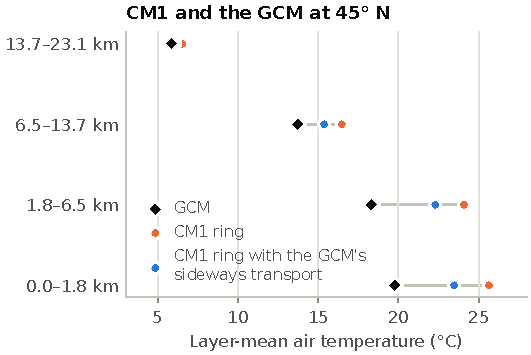
\includegraphics[width=0.62\textwidth]{figures/fig_gap.pdf}
\caption{Layer-mean air temperature over the second lunar day on the 45\textdegree\,N ring: CM1 alone, CM1
with the GCM's transport across the circle imposed, and the GCM's design case on the same row, years
10--19. The imposed transport removes 2.2 of the 5.9~K warm offset in the lowest 1.8~km, 37\%.}
\label{fig:gap}
\end{figure}

\textbf{Storms and lightning.} At lunar gravity the 0\,\textdegree C and $-40$\,\textdegree C levels stand
five to six times higher than in Earth's tropics, near 25 and 60~km, and cloud tops reach
55--80~km.\claim{G09} The lightning the storms make is rarer and larger than Earth's. The main electrified
run, two lunar days of a box at 0\textdegree~E forced from the GCM before its corrections, made 530
flashes, 0.022 per square kilometre per year, about a hundredth of Earth's average; up to a fifth were
negative ground strikes, counted under WRF-ELEC's rule with the leader's crossing, an upper bound, and none
was positive. Each ground strike lowered a median 149~C where Earth's lower 5--30~C, while in-cloud flashes
neutralised a median 108~C. The charge keeps Earth's arrangement at five to six times its height: flashes
start a median 35.8~km up, and the main negative charge sits at 40--42~km, at $-13$ to $-14$\,\textdegree C,
just above the $-7$\,\textdegree C level as on Earth. Hail, which rimes faster than the lunar graupel, does
87\% of the non-inductive charging.\claim{G10}

Two of the storm results hang on choices that measurement or theory could settle. Under Takahashi's charging
law \autocite{takahashi1978riming} in place of Saunders and Peck's \autocite{saunders1998laboratory} the
storms separate as much charge with their polarity inverted, so the lightning's sign rests on laboratory laws
that disagree on the sign rimed ice takes in the little cloud water of the lunar storms; and with the NSSL
microphysics in place of Morrison's the same box runs 1.0~\textdegree C warmer at 2~m and its night fog at the
ground covers 29\% of the box in place of 56\%, so the lunar night fog depends on the microphysics by about a
factor of two.\claim{G11}

\textbf{Seas.} Forced by sixty days of the GCM's surface stress, SWAN finds the light lunar winds raising
big, slow waves: the same wind, fetch and duration build waves 4--5 times as high as on Earth, with periods
five times as long. Over the nearside sea, 5.29 million~km$^2$, the mean significant wave height is 1.39~m,
68\% of area and time stands at or above 1~m, and the largest sea reaches 4.9~m with a 19.3~s mean period.
Lunar waves keep Earth's steepness and travel at 0.41 of the speed of an Earth wave of the same length.
SWASH runs them up today's steep slopes to a 98th-percentile run-up of 2.1~m on the exposed face of the
eastern Smythii headland.\claim{G12} These wave results rest on the corrected design climate as it stood
before the curved air and the gas bands, and on Earth's laws for wind input, whitecapping and breaking.

\textbf{What stays conditional.} The conditions under these numbers differ in weight. The design temperature
of 295~K is a target held by dimming the sunlight; the 307~K state of the longwave test is a sensitivity
resting on a correction used beyond its fit. The warmth and humidity of the air near the ground, the air
people would live in, stand best as a range between the models, 3.7~K wide in the lowest 1.8~km at
45\textdegree\,N with the GCM's transport imposed and against the GCM before its longwave correction. The
lunar rain depends on a convection scheme fitted to Earth in the GCM and on Earth's drop limits in CM1, the
lightning's polarity on a laboratory charging law, and the seas on Earth's wave physics carried to lunar
gravity by similarity.
